\documentclass[12pt]{article}
\usepackage{graphicx}
\usepackage{caption}
\usepackage[multiple]{footmisc}
\usepackage{cleveref}
\usepackage{lipsum}
\usepackage{wrapfig}
\usepackage{subfig}
\usepackage{tabularx}
\usepackage[T1]{fontenc}
\usepackage{amsmath}
\usepackage{fixltx2e}
\usepackage[font=scriptsize,labelfont=bf]{caption}
\crefformat{footnote}{#2\footnotemark[#1]#3}
\title{\textbf{Action selection - Guthrie Model}}
\author{Bhargav Teja Nallapu}
\begin{document}

\begin{figure}[ht]
  \centering
  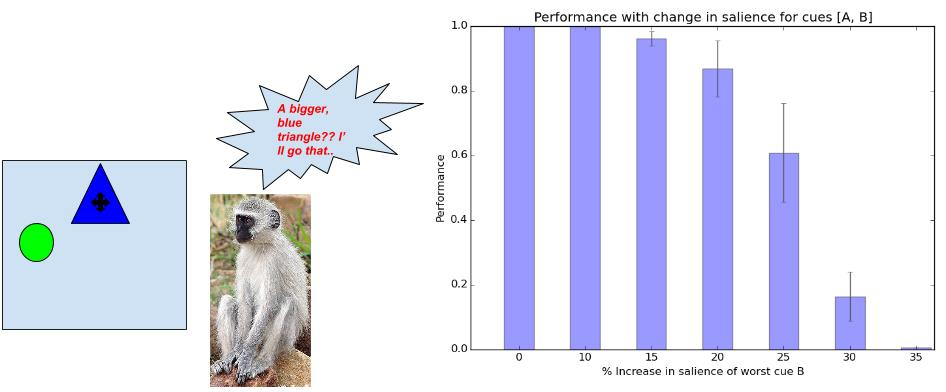
\includegraphics[width=\textwidth]{MonkeyTask_21.jpg}
  \caption[Varying performance under external factors]{Cue 'A' has the best rewarding probability of 1 and cue 'B' is less rewarding, with a probability of 0.33. \emph{The model} is correct if it selects A when presented with A,B. When stimulus B is presented with higher salience than A, the performance of \emph{of the model} decreases as salience of B increases. It can be observed that when the salience of B is 30\% more than that of A, performance of the \emph{model} decreases to as low as 0.20}
\end{figure}

\clearpage

\begin{figure}[ht]
  \centering
  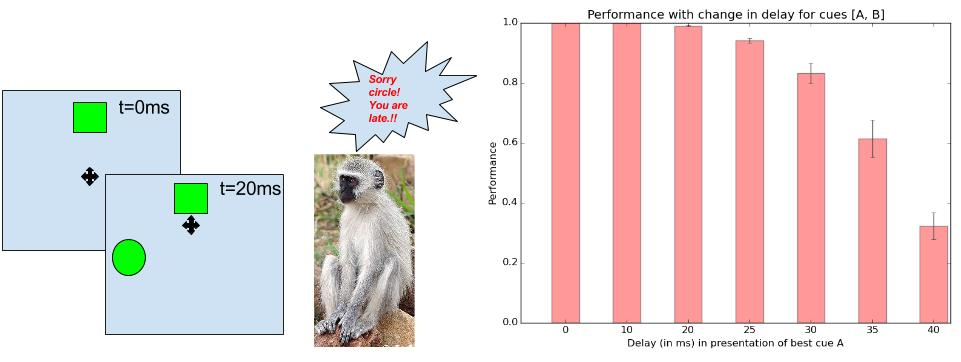
\includegraphics[width=\textwidth]{MonkeyTask_31.jpg}
  \caption[Varying performance under external factors]{Cue 'A' has the best rewarding probability of 1 and cue 'B' is less rewarding, with a probability of 0.33. \emph{The model} is correct if it selects A when presented with A,B. When only stimulus B is presented at first, then after a certain delay stimulus A is presented, the performance of the \emph{model} decreases as the delay increases.}
\end{figure}

\nocite{*}
\bibliography{decisionmaking.bib}{}
\bibliographystyle{plain}

\end{document}